\chapter{Feature Detection and Correspondance}

In this section we explain how feature points are detected and matched between
different camera frames. The common feature detection and matching pipeline for
localization and mapping algorithms is:

\begin{enumerate}
  \setlength{\itemsep}{0pt}
  \setlength{\parskip}{0pt}
  \setlength{\parsep}{0pt}
  \item{Detect regions of interests (image feature) in the image}
  \item{Extract image feature information using descriptors}
  \item{Match extracted descriptors}
\end{enumerate}



\section{FAST}
\label{sec:fast}

Feature detection in computer vision is a process of gathering scene
information and deciding locally whether an image feature exists. The resulting
subset of image features in the image domain can in turn be used for
localization and mapping algorithms to estimate the camera pose.

For our requirements corners was the chosen image feature. The most widely used
corner detector is the FAST feature detector~\cite{Rosten2006}. The advantage
of using FAST includes its speed and high detection rate. It operates by
inspecting a gray-scale image and applying a Bresenham circle or patch of
configurable radius (radius of 3 for a 16 pixel circle in
Fig~\ref{fig:fast_corner}), where each pixel value on the circle is labeled
clockwise. If a set of $N$ contiguous pixels in the circle are all brighter
than the intensity of the center candidate pixel $p$ plus a threshold value
$t$, or are all darker compared to $p$ minus a threshold value $t$, then $p$ is
considered a corner.

\begin{figure}[h]
  \centering
  \includegraphics[width=0.6\linewidth]{images/feature/fast.jpg}
  \caption{FAST Corner Detection~\cite{Rosten2006}}
  \label{fig:fast_corner}
\end{figure}

% A uniform feature distribution over the image domain is known to avoid
% degenerate configurations for SLAM, and reduce redundant information. Further,
% a uniform and un-clustered corner distribution has the potential of increasing
% computer vision pipeline efficiency, as a lower number of features are required
% for the whole image. To encourage a uniform feature distribution a custom naive
% implementation of Grid-FAST was implemented~\footnote{At the time of writing
% OpenCV has removed the interface to the \texttt{GridAdaptedFeatureDetector}
% implementation from their code base.}. The naive Grid-FAST was implemented as
% follows, given an image we divide the image into $r$ rows and $c$ columns with
% the goal of detecting a total max number of $N$ corners. The max number of
% corners per grid cell $n$ is then given as
% %
% \begin{equation}
% n = \dfrac{N}{r \times c}.
% \end{equation}
% %
% Using $n$ we limit the corners detected in each image grid cell to naively
% encourage a uniform distribution.
%
% \begin{figure}[H]
%   \centering
%   \begin{subfigure}{0.47\textwidth}
%     \centering
%     \includegraphics[width=\linewidth]{images/background/fast.png}
%     \caption{FAST Detection (1000 Corners)}
%   \end{subfigure}
%   \hspace{0.5em}
%   \begin{subfigure}{0.47\textwidth}
%     \centering
%     \includegraphics[width=\linewidth]{images/background/grid_fast.png}
%     \caption{Grid-FAST Detection (714 Corners)}
%   \end{subfigure} \\ \vspace{1.0em}
%   \begin{subfigure}{0.485\textwidth}
%     \centering
%     \includegraphics[width=\linewidth]{images/background/fast_hist2d.png}
%     \caption{2D Histogram of FAST Detection}
%     \label{subfig:fast_hist2d}
%   \end{subfigure}
%   \hspace{0.3em}
%   \begin{subfigure}{0.485\textwidth}
%     \centering
%     \includegraphics[width=\linewidth]{images/background/grid_fast_hist2d.png}
%     \caption{2D Histogram of Grid-FAST Detection}
%     \label{subfig:grid_fast_hist2d}
%   \end{subfigure}
%   \caption{Comparison between FAST and Grid-FAST}
%   \label{fig:grid_fast_comparison}
% \end{figure}
%
% In Fig.~\ref{fig:grid_fast_comparison} both FAST and Grid-FAST observe the same
% image scene with the same detection parameters. Grid-FAST divided the image
% into 10 rows and columns to encourage a uniform corner detection. While
% Grid-FAST detected a lower number of corners compared to FAST (714, 1000
% respectively), we can observe the benefit of using Grid-FAST in
% Fig.~\ref{subfig:fast_hist2d} and Fig.~\ref{subfig:grid_fast_hist2d}, where it
% clearly shows that FAST detection has an undesirably high detection
% concentration around the chessboard in this particular scene, Grid-FAST on the
% other hand does not exhibit the same problem. Although, Grid-FAST obtains
% features of lower quality in terms of repeatable detection, the threshold of
% corner-ness can be increased if this is an issue.



\section{ORB Feature Descriptor and Matching}
\label{sec:orb}

To correspond image features detected in two different image frames a feature
descriptor is used. Feature descriptors are a way to describe the image feature
observed for matching. There are a number of feature descriptors that extract
patch information in order to create a robust and repeatable match. Feature
descriptors such as SIFT~\cite{Lowe1999}, SURF~\cite{Bay2006}, are histogram of
gradients (HOG) based patch descriptors. These HOG descriptors are invariant to
small rotations and lighting variations, they are however, relatively expensive
to compute. The computationally expensive components are its calculation of the
image gradient and large descriptor dimension. While both descriptors provide
quality information of image features, the aforementioned computational factors
impact the matching speed significantly.

Binary descriptors such as BRIEF~\cite{Calonder2010}, ORB~\cite{Rublee2011} and
BRISK~\cite{Leutenegger2011} have been proposed to speed up the feature
descriptor and matching process. The performance boost in binary descriptors
comes in the form of using a binary sampling pattern around each image feature
previously detected (see Fig~\ref{fig:binary_descriptors}), and outputting a
binary vector, instead of computing image gradients and outputting a floating
point vector. Each binary descriptor uses its own unique sampling pattern, and
outputs a binary string to be used for matching. The matching process is
cheaper compared to the HOG based descriptors, because instead of comparing two
floating point vectors, comparing binary descriptors is performed by computing
the Hamming distance using a XOR or bit count operation, which can be performed
extremely quickly on modern CPUs~\cite{Calonder2012}.

\begin{figure}[htp]
  \centering
  \begin{subfigure}[t]{0.31\textwidth}
    \centering
    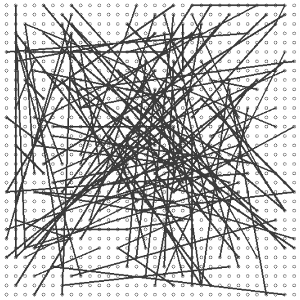
\includegraphics[width=\linewidth]{images/feature/brief.png}
    \caption{BRIEF Descriptor~\cite{Calonder2012}}
  \end{subfigure}
  \begin{subfigure}[t]{0.33\textwidth}
    \centering
    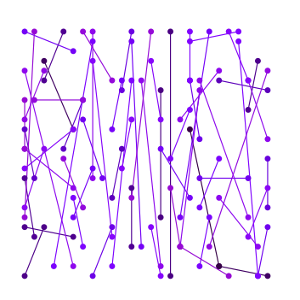
\includegraphics[width=\linewidth]{images/feature/orb.png}
    \caption{ORB Descriptor~\cite{Rublee2011}}
  \end{subfigure}
  \begin{subfigure}[t]{0.31\textwidth}
    \centering
    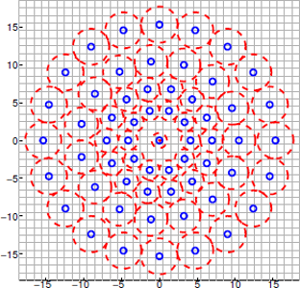
\includegraphics[width=\linewidth]{images/feature/brisk.png}
    \caption{BRISK Descriptor~\cite{Leutenegger2011}}
  \end{subfigure}
  \caption{Binary Descriptors}
  \label{fig:binary_descriptors}
\end{figure}

% \begin{figure}[htp]
% 	\centering
% 	\begin{subfigure}[t]{0.45\textwidth}
% 		\centering
% 		\includegraphics[width=\linewidth]{images/background/orb_matches1.png}
% 	\end{subfigure}
% 	\hspace{1.0em}
% 	\begin{subfigure}[t]{0.45\textwidth}
% 		\centering
% 		\includegraphics[width=\linewidth]{images/background/orb_matches2.png}
% 	\end{subfigure}
% 	\caption{ORB descriptors detecting features in the EuRoC MAV dataset~\cite{Burri2016}}
% 	\label{fig:orb_descriptors_in_action}
% \end{figure}
%
% Following~\cite{Shelly2014}, the ORB descriptor was chosen for experimentation.
% The ORB descriptor is considered as an improvement over BRIEF with the addition
% of being orientation invariant. However, it can be observed in
% Fig.~\ref{fig:orb_descriptors_in_action} that the ORB detector from OpenCV
% strongly favours strong corners over keeping the detected points uniform over
% the image space. As a result the key-points are mostly clustered around the
% chessboard observed in the scene. This is in contrast to Grid-FAST discussed in
% Section.~\ref{subsec:fast_feature_detection}, where the features detected are
% uniformly distributed over the entire image space. Because of ORB features not
% being uniformly distributed, the KLT feature tracker is considered and is
% discussed in the following section.



\section{KLT Feature Tracker}
\label{sec:klt}

In the previous section, we showed how ORB descriptors and matching methods are
used to correspond and match features across multiple camera frames. This
process of corresponding the the same features across multiple camera frames is
called feature tracking. There are many different feature tracking pipelines.
Matching feature descriptors such as ORB has shown to have better temporal
tracking accuracy compared to KLT-based methods~\cite{Paul2017}. However, in
the work of~\cite{Sun2018}, descriptor-based feature trackers were found to
require more computational resources with limited gains in tracking accuracy.
Making it less attractive for real-time operation. In the following we will
briefly describe the KLT feature tracker, but first an understanding of optical
flow is required.


\subsubsection{Optical Flow}

Optical flow estimates the velocity of each image feature in successive images
of a scene. It makes the following explicit assumptions:

\begin{itemize}
  \setlength{\itemsep}{1pt}
  \setlength{\parskip}{0pt}
  \setlength{\parsep}{0pt}

  \item{Pixel intensity does not change between consecutive frames}
  \item{Displacement of features is small}
  \item{Features are within the same local neighbourhood}
\end{itemize}

Let us consider a pixel, $p$, in the first frame which has an intensity, $I(x,
y, t)$, where it is a function of the pixel location, $x$ and $y$, and time,
$t$. If we apply the aforementioned assumptions, we can say that the intensity
of said pixel in the first frame to the second does not change. Additionally,
if there was a small displacement, $dx$ and $dy$, and small time difference,
$dt$, between images this can be written in mathematical form as,
%
\begin{equation}
  \label{eq:brightness_constancy}
  I(x, y, t) = I(x + dx, y + dy, t + dt).
\end{equation}
%
This is known as the brightness constancy equation. To obtain the image
gradient and velocity of the pixel, we can use Taylor series approximation of
right-hand side of Eq.~\eqref{eq:brightness_constancy} to get,
%
\begin{equation}
  I(x + dx, y + dy, t + dt) = I(x, y, t)
    + \dfrac{\partial{I}}{\partial{x}} dx
    + \dfrac{\partial{I}}{\partial{y}} dy
    + \dfrac{\partial{I}}{\partial{t}} dt
    + \text{H.O.T},
\end{equation}
%
removing common terms and dividing by $dt$ we get,
%
\begin{equation}
  \label{eq:optical_flow}
  I_{x} v_{x} + I_{y} v_y + I_{t} = 0
\end{equation}
or,
%
\begin{equation}
  \label{eq:optical_flow_2}
  I_{x} v_{x} + I_{y} v_y = -I_{t}
\end{equation}
%
where:
%
\begin{align}
  I_{x} = \dfrac{\partial I}{\partial x}
  ; \quad
  I_{y} = \dfrac{\partial I}{\partial y} \nonumber \\
  v_{x} = \dfrac{dx}{dt}
  ; \quad
  v_y = \dfrac{dy}{dt}. \nonumber
\end{align}
%
The image gradients along the x and y directions are $I_{x}$ and $I_{y}$, where
$I_{t}$ is the image gradient along time, finally, $v_{x}$ and $v_{y}$ are the
pixel velocity in $x$ and $y$ directions, which is unknown. The problem with
Eq.~\ref{eq:optical_flow_2} is that it provides a single constraint with two
degrees of freedom, and as such requires at least one additional constraint to
identify a solution.

The Lucas-Kanade method solves the aperture problem by introducing additional
conditions. This method assumes all pixels within a window centered around a
pixel $p$ will have similar motion, and that the window size is configurable.
For example, a window size of $3 \times 3$ around the pixel $p$, the $9$ points
within the window should have a similar motion. Using
Eq.~\ref{eq:optical_flow_2}, the intensity inside the window must therefore
satisfy,
%
\begin{align}
  I_{x}(p_1) v_{x}(p_1) &+ I_{y}(p_1) v_y = -I_{t}(p_1) \nonumber \\
  I_{x}(p_1) v_{x}(p_2) &+ I_{y}(p_2) v_y = -I_{t}(p_2) \nonumber \\
  & \enspace \vdots \nonumber \\
  I_{x}(p_1) v_{x}(p_n) &+ I_{y}(p_n) v_y = -I_{t}(p_n) \nonumber
\end{align}
%
where $p_{1}, p_{2} ,\dots , p_{n}$ are the pixels in the window. This can be
re-written in matrix form $\mathbf{A} \mathbf{x} = \mathbf{b}$ as,
%
\begin{equation}
  \label{eq:lucas_kanade_1}
    \mathbf{A} = \begin{bmatrix}
        I_{x}(p_{1}) & I_{y}(p_{1}) \\
        I_{x}(p_{2}) & I_{y}(p_{2}) \\
        \vdots & \vdots \\
        I_{x}(p_{n}) & I_{y}(p_{n})
    \end{bmatrix}
    \quad
    \mathbf{x} = \begin{bmatrix}
      v_{x} \\ v_{y} \\
    \end{bmatrix}
    \quad
    \mathbf{b} = \begin{bmatrix}
      -I_{t}(p_{1}) \\
      -I_{t}(p_{2}) \\
      \vdots \\
      -I_{t}(p_{n})
    \end{bmatrix}.
\end{equation}
%
The linear system of equations of Eq.~\ref{eq:lucas_kanade_1} is
over-determined, therefore there is no exact solution. To address this issue, a
least squares method can be used to approximate the solution by applying the
ordinary least squares. For the system $\mathbf{A} \mathbf{x} = \mathbf{b}$,
the least squares formula is obtained by minimizing the following,
%
\begin{equation}
  \underset{\mathbf{x}}{\text{argmin }} || \mathbf{A} \mathbf{x} - \mathbf{b} ||,
\end{equation}
%
the solution of which can be obtained by using \textit{normal equations},
%
\begin{align}
  \label{eq:normal_equations_1}
  \mathbf{A}^{T} \mathbf{A} \mathbf{x} &= \mathbf{A}^{T} \mathbf{b} \\
  \label{eq:normal_equations_2}
  \mathbf{x} &= (\mathbf{A}^{T} \mathbf{A})^{-1} \mathbf{A}^{T} \mathbf{b}.
\end{align}
%
Rewriting Eq~\ref{eq:lucas_kanade_1} in the form of Eq.~\ref{eq:normal_equations_2} we get,
%
\begin{equation}
  \begin{bmatrix}
  v_{x} \\ v_{y}
  \end{bmatrix}
  =
  \begin{bmatrix}
    \sum_{i}{I_{x}(p_{i})}^2 & \sum_{i}{I_{x}(p_{i}) I_{y}(p_{i}) } \\ 
    \sum_{i}{I_{x}(p_{i}) I_{y}(p_{i})} & \sum_{i}{I_{y}(p_{i})}^2
  \end{bmatrix}^{-1}
  \begin{bmatrix}
    - \sum_{i}{I_{x}(p_{i}) I_{t}(p_{i})} \\ 
    - \sum_{i}{I_{y}(p_{i}) I_{t}(p_{i})}
  \end{bmatrix}
\end{equation}
%
which is finally used to obtain the optical flow of pixel $p$.

% \begin{figure}[H]
% 	\centering
% 	\begin{subfigure}[t]{0.47\textwidth}
% 		\centering
% 		\includegraphics[width=\linewidth]{images/background/klt_matches1.png}
% 	\end{subfigure}
% 	\hspace{1.0em}
% 	\begin{subfigure}[t]{0.47\textwidth}
% 		\centering
% 		\includegraphics[width=\linewidth]{images/background/klt_matches2.png}
% 	\end{subfigure}
% 	\caption{KLT Feature Tracker in Action}
% 	\label{fig:klt_in_action}
% \end{figure}


\subsubsection{KLT Feature Tracker}

The Lucas-Kanade method recovers feature pixel velocities from consecutive
camera frames. The issue with the Lucas-Kanade method is that it assumes the
features detected have small displacements between consecutive camera frames.
Therefore to track features that have a large motion the Kanade-Lucas-Tomasi
(KLT) feature tracker~\cite{Lucas1981} uses reduced-scale versions of the input
images in order to track features over multiple camera frames. The general
steps of the KLT feature tracker is as follows,
%
\begin{enumerate}
	\item{Detect corners in the first camera frame}
	\item{For each corners, compute the motion between consecutive camera frames
			  using a pyramidal implementation of the Lucas-Kanade method}
	\item{Match motion vectors between consecutive camera frames to track corners}
	\item{Detect new corners if number of tracks currently tracking is too low}
	\item{Repeat steps 2 to 4}
\end{enumerate}
